\documentclass[11pt]{article}

\title{This is an Essay}
\author{Bert Baumgaertner and James A. Overton}
\date{}

\usepackage{geometry}
\usepackage{amsmath, amsfonts, amssymb, amsthm, mathrsfs}
%\usepackage{hyperref}
%\usepackage{natbib}
\usepackage{graphicx, tikz}
%\usepackage{fitch}
\usepackage{setspace}
%\usepackage{algorithmic, algorithm}

%\usepackage[small,nohug,heads=littlevee]{diagrams} 
%\diagramstyle[labelstyle=\scriptstyle] 

\newcommand{\N}{\mathbb{N}}
\newcommand{\NN}{{\rm NN}}
\newcommand{\Her}{{\rm Her}}
\newcommand{\defined}{=_{df}}
\newcommand{\la}{\leftarrow}
\newcommand{\ra}{\rightarrow}
\newcommand{\lra}{\leftrightarrow}
\newcommand{\Ra}{\Rightarrow}
\newcommand{\La}{\Leftarrow}
\newcommand{\imp}{\supset}
\renewcommand{\iff}{\leftrightarrow}
\newcommand{\IFF}{\Leftrightarrow}
\renewcommand{\L}{\mathcal{L}}
\newcommand{\n}{\mathfrak{N}}
\newcommand{\Th}{{\rm Th}}
\newcommand{\Craig}{{\rm Craig}}
\renewcommand{\phi}{\varphi}


%\newenvironment{itemize*}{
%\begin{itemize}
% \setlength{\itemsep}{1pt}
% \setlength{\parskip}{0pt}
% \setlength{\parsep}{0pt}
% \singlespacing
%}{\end{itemize}\doublespacing}
%\newenvironment{description*}{
%\begin{description}
% \setlength{\itemsep}{1pt}
% \setlength{\parskip}{0pt}
% \setlength{\parsep}{0pt}
% \singlespacing
%}{\end{description}\doublespacing}
%\newenvironment{enumerate*}{
%\begin{enumerate}
% \setlength{\itemsep}{1pt}
% \setlength{\parskip}{0pt}
% \setlength{\parsep}{0pt}
% \singlespacing
%}{\end{enumerate}\doublespacing}
%\newenvironment{quote*}{
%\begin{quote}
% \singlespacing
%}{\end{quote}\doublespacing}

\begin{document}

%\maketitle
%\tableofcontents
%\newpage
%\doublspacing
%\onehalfspacing




\section{Introduction}

% Say something about the history of mathematical and computation modelling in biology? Where to start?

The Lotka-Volterra equations for predator-prey relationships are well-known and striking examples of mathematical modelling in biology. The model works \emph{top-down} by describing populations directly, abstracting away from details about the individuals that make up the populations. In the hundred years since Lotka proposed his equations, biologists have made increasing use of \emph{bottom-up} models that start from individuals, and in which interesting properties of populations sometimes \emph{emerge}. Increasing computer power allows for larger and more detailed models, and for batches of simulations that explore the space of model parameters. In this paper we discuss the increasingly popular class of `agent-based models' (ABMs), characterize a group of `mixed-level' ABMs, and consider what mixed-level ABMs can teach us about reduction and emergence.

% Is GoL a model? Of what? Is it a simulation? Of what?

Conway's Game of Life is a particularly good example of a bottom-up model with rich emergent patterns. We start with a grid of cells that are either white (OFF) or black (ON) and a handful of rules that determines whether a cell maintains or changes its state in the next time-step, depending entirely upon the states of its immediate neighbours in the current time-step.  Despite its wonderful simplicity, a number of complicated behaviours or patterns can be recognized when a simulation is seeded with particular arrangements of OFF and ON cells.  One of the most common patterns is a \emph{glider}, an `object' that moves diagonally across the grid.  Strictly speaking, however, the Game of Life doesn't recognize or encode such `objects' -- you won't find them written into the computer code. Rather, gliders and other macro-level patterns `emerge out of' the simulation dynamics of the Game of Life (when seeded with certain configurations). Put another way, the macro-level patterns can be `reduced to' the micro-level: a macro-level description of a glider can be fully accounted for by a micro-level description of transitions between cell states.  In this paper we will regard Conway's Game of Life as a paradigm example of a `bottom-up' model. 

% A figure of GoL might be useful.

%What happens at the aggregate level is wholly determined by interactions between neighbouring cells.  [MENTION INDIVIDUALISM?]

Conway's Game of Life belongs to a larger class of discrete mathematical models called `cellular automata'. Agent-based models are in many respects similar to cellular automata, but with fewer constraints. ABMs consist of three main elements: agents, an environment, and interactions (agent-agent and agent-environment). The environment is not limited to a grid, although a two-dimensional grid is often used. It could be a grid with additional information about `altitude' or energy gradients, or a more abstract network that connects agents. Each agent usually has more `state' than a cell in a cellular automaton. Agents often have a `location`, an `age', an `energy level', and other parameters by which they differ from their peers. The interaction rules between agents and between agents and their environment can take advantage of this additional complexity, making use of each agent's distinct parameters and the constraints on interactions imposed by the environment. Time can be discrete, as in cellular automata, or it can be continuous.

Just as state transitions of cells in the Game of Life can produce macro-level patterns, agents in an ABM can give rise to group behaviour \emph{without} having to posit the existence of groups in the model.  A Lotka-Volterra model is explicitly about group-level properties or patterns. Agent-based models, on the other hand, focus on individuals and their interactions between one another and their environment.  This leads us to consider agent-based models to be another example of a `bottom-up' model; what happens at the aggregate level is wholly determined by agent-agent and agent-environment interactions -- no mention of groups required.

% Need to cite the ant ABM.

The classic ant foraging ABM demonstrates how biologically interesting patterns can emerge from simple interactions between a collection of agents. The environment is a two-dimensional grid that also contains information about the location of food sources and the level of `pheremones` at each cell in the grid. The agents are `ants' that walk around the grid searching for food. If they find food they return to their nest, emitting at each step a pheremone that remains at that location and slowly degrades. Other ants can detect the pheremone, and will move toward higher concentrations. The simulation begins with ants wandering randomly across the environment, but quickly shifts to striking organized behaviour a few ants randomly discover food, then others follow their trail, forming a highway between the nest and the food source. Similar to the Game of Life, each ant only has information about its immediate surroundings, but this information is enough for complex path-following behaviour to emerge.

Ant foraging shows how ABMs can be bottom-up and demonstrate emergence. There are many similar examples. This has led to a common view that ABMs as a group are bottom-up. We argue that this conception is misleading. It is usually better to think of ABMs as mixed-level.

To illustrate we consider a case that invites us to take seriously population- or group-level selection.  The case we will look at is how individual \emph{E.Coli} bacteria in a group seem to have `coordinated'  their rates of fimbriation (hair-like structures on cell walls) with one another so that: i) they avoid triggering an immune response by their host, but ii) still have a high enough virulence level to cause the production of sialic acid (a source of nutrients).  Unlike many other group-level phenomena, such `coordination' is presumably not driven by social dilemmas that give rise to, e.g. cooperation.\footnote{Examples of social dilemmas that have been modeled include the stag hunt and the prisoner's dilemma [CITE Brian Skryms and Robert Axelrod].}  Without these social dilemmas, it is unlikely that a social structure would evolve as a means to solve the problem. So, one might object that the best way to proceed is to reinterpret what's happening in the \emph{E.coli} case by focusing only on the individual bacteria and their interactions. As a proof of this possibility, one could attempt to use an ABM approach to see how far the population phenomenon can be reduced to -- or emerge out of -- individuals and their interactions with one another. However, we will show how a seemingly promising attempt to do this explicitly represents interactions between population-level properties and individual-level interactions, and hence is a mixed-level model (as opposed to strictly `bottom-up'). We find this not so surprising given that there are independent reasons for thinking that selection can't be operating at the level of individuals: since the fate of one individual is tied to all the others in their group, variation in a group can't be doing the relevant explanatory work.

The \emph{E.coli} example shows that there are places where ABMs invite the introduction of macro-level properties.  We do not, however, believe that this occurs because of the particular subject matter for which an ABM is being used. Rather, we argue that there are particular features of ABMs that are particularly susceptible to representing macro-level properties, features that distinguish ABMs from their cousins -- cellular automata. These include: the environment, agent-agent interactions, and agent-environment interactions.  Because these features make representing macro-level properties readily accessible (whereas the features of cellular automata do not) we argue that ABMs are better conceived of as mixed-level.

We also argue that conceiving of agent-based models this way gives us a better philosophical understanding of their epistemological role in science.  The biological sciences, like many others, tend to proceed by methodological reduction. That is, they attempt to understand a phenomenon by breaking it down into organized parts that interact with one another.\footnote{The new mechanists have picked up on this strategy and have developed philosophical counts. See CITE}  Models can be used to get a first approximation of the phenomenon, and then can be revised to reflect further ideas about how the phenomenon can be reduced. In the meantime, however, the models may have to illicitly appeal to features of the very phenomenon they attempt to reduce. In this way, models, especially agent-based models, can provide the scaffolding for the development of a model that is `purely' bottom-up.  We think that this is an appealing feature of ABMs and is well captured by the view that ABMs are better conceived of as mixed-level models.

\section{Evolution of optimal \emph{E.coli} fimbriation levels}

Agent-based models are becoming increasingly popular in the biological sciences. In this section we explain one such example. What it will highlight is that ABMs can easily be used to model multiple levels, and that this is one of their advantages. We draw on the work of (CITE Barnes and Chu)


\subsection{Target Phenomenon}

Fimbriae are hair-like structures that grow on bacteria like \emph{Escherichia coli} (\emph{E.coli} for short).  These structures allow bacteria to hold on to hosts cells.  Although it is not always the case, fimbriae can have a virulence factor. It is well known, for example, that some non-disease causing (`commensal') strains of \emph{E.coli} are found in the gastro-intestinal tracts of humans.\footnote{More information about \emph{E.coli} can be found at CITE (Escherichia coli 2013, CDC National Center for Emerging and Zoonotic Infectious Diseases)}  The virulence factor of these bacteria turns out to be very low, where what is mean by `low' is that a small proportion of the population is expressing fimbriae.

What is particularly interesting about these fimbriation levels has to do with the relationship between the bacteria and their host. As long as the fimbriation levels aren't too high, the host produces an amount of sialic acid that is proportional to the level of fimbriation. This turns out to be a good thing for the bacteria, because sialic acid can be a source of nutrients. However, if the fimbriation levels exceed a certain threshold, then an immune response is triggered and the entire population is knocked out. So the question that interests scientists is how populations of \emph{E.coli} manage to coordinate their fimbriation rates so that they come close to optimal levels without going over the edge. This requires understanding some of the mechanisms involved in the expression of fimbriae.

The expression of fimbriae is guided by the \emph{fim} operon. It contains an invertible element called \emph{fimS}. If it is in the ON-orientation then the cell expresses fimbriae, if \emph{fimS} is in the OFF-orientation then the cells does not. There are two proteins involved in the orientation of \emph{fimS}. These are FimB and FimE. FimB tends to switch \emph{fimS} back and forth at relatively equal rates. FimE, on the other hand, tends to switch \emph{fimS} from ON to OFF , and it does so at a faster rate than FimB.  So effectively, FimB is what turns fimbriation on, wherease FimE is what turns it off.  And whether more or less of each of these proteins are around will depend on the level of sialic acid in the cell's environment.  This is where there can be variation across individual bacteria - some of them will have faster switching rates than others at different levels of sialic acid concentration.

Since every cell can take up sialic acid whether or not it is expressing fimbriae, one of the main questions biologists are asking is how these rates of fimbriation could have evolved to roughly optimal levels (CITE Shaikh et al 2007).  There is no evidence to suggest that the bacteria are able to communicate with one another. Moreover, it is unlikely that their `coordination' could have evolved by selection pressures on variation across individuals, since the fate of each individual is tied to the fate of the group.\footnote{CITE Feldgarden et al 2003 for further discussion of \emph{E.coli} and selection.} The most plausible mechanism seems to be group selection.

The idea is as follows. Inevitably every host is colonized with some population of \emph{E.coli}, so even if a host gets sick and eliminates a colony, they will eventually be recolonized by a new population of \emph{E.coli}.  This new colony will tend to be genetically homogenous compared to the genetic heterogeneity across populations of \emph{E.coli} in different hosts. This is because, despite some weak interaction between different populations of \emph{E.coli}, there is a strong \emph{founder effect} -- new populations initially have less genetic variation from where they came from. So the group selection idea is this: the re-colonization of a host is the equivalent of reproduction; mutation within a population and weak migration are the group-level equivalents of mutation; and the elimination of populations by hosts provide the selection pressures. So, those populations that are bigger and last longer have more opportunities to migrate and recolonize hosts. This creates competition. One group is fitter than another if they have a larger population and are less likely to become extinct. The result is that populations will tend to evolve that are closer to optimal levels of fimbriation.(CITE Barnes and Chu again?)

This verbal model leaves many details to be considered, and that is often where the devil lurks. So to test the plausibility of this explanation, researchers have used agent-based models as a way to give a more rigorous characterization of the proposal. The models can then be simulated to generate data, which in turn can be compared to empirical results.

\subsection{An ABM of Evolving Fimbriation Levels}

In Figure \ref{abmalg} is the pseudo-code of the agent-based model we will be referring to.
[WE'LL NEED TO FIGURE OUT HOW MUCH WE NEED TO SAY]

\begin{figure}
\label{abmalg}
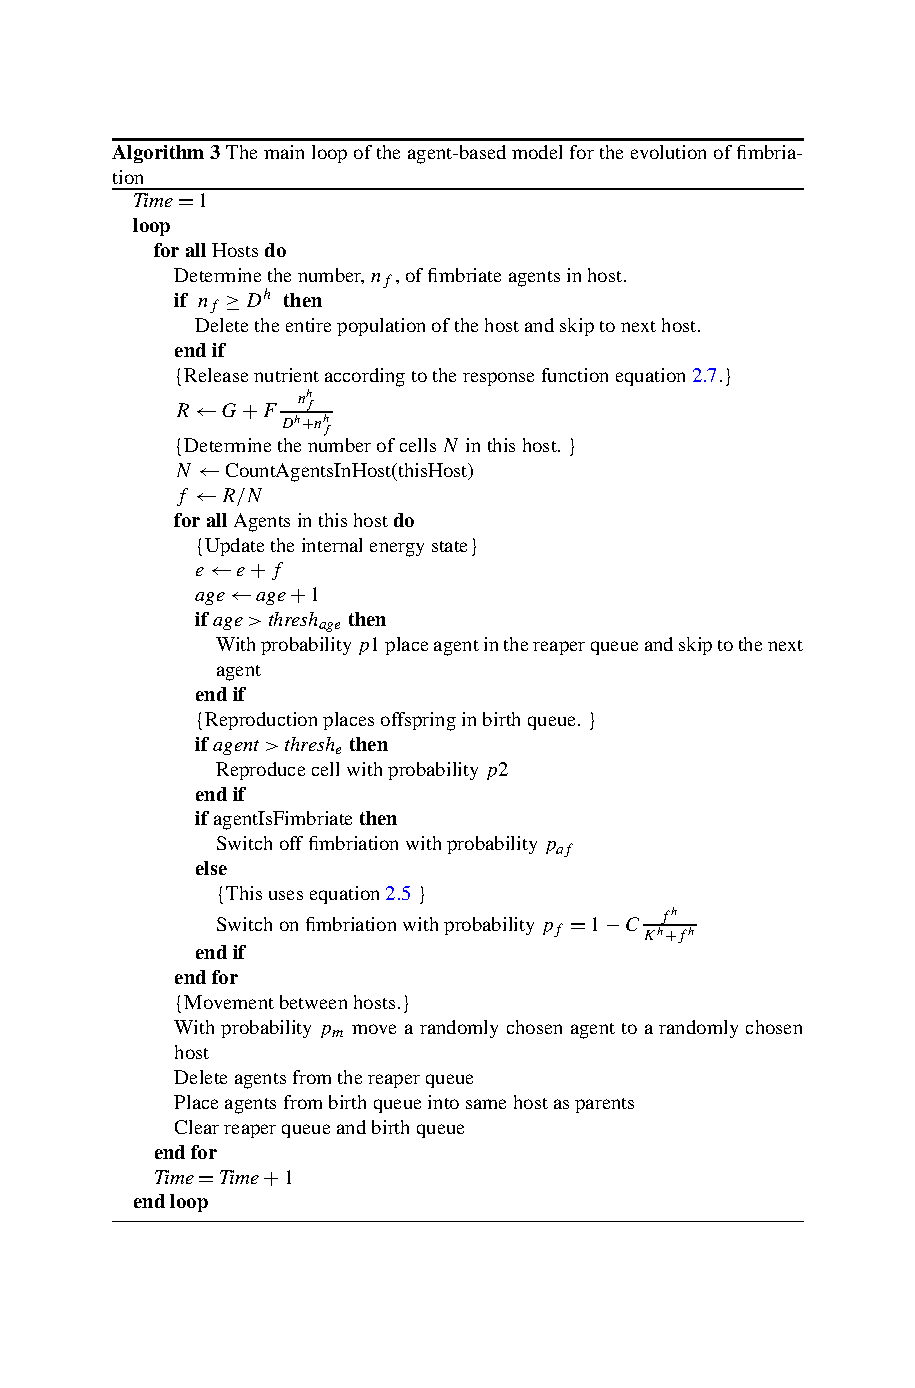
\includegraphics[width = 4.5in]{abmofevofimalgorithm}
\caption{Taken from Barnes and Chu}
\end{figure}

There are several places in the algorithm where aggregated information is used. We do not take this to be by itself problematic.  To explain why, it is helpful to contrast this example with Conway's Game of Life. Recall that in order to decide whether to turn ON or OFF at the next time step, a cell looks at how many of its eight neighbours are ON. This involves the aggregation of information, which can be expressed as a property of a group. For example, if 4 of a cell's neighbours are ON, that can be express by saying `half of the neighbourhood is ON'. Although we can imagine that someone might already take this to be problematic, we think this is too nit-picky.  The better place to focus is the relationship between cells and the emergent patterns.

The spirit in which the Game of Life is designed is that objects that sit at the higher-level of organization, such as gliders and eaters, do not interact with the cells at the lower-level of organization.  Whatever `causal efficacy' a glider has is fully exhausted by the causal efficacy of its constituents. Gliders aren't intended to be part of the underlying code, they simply `arise' as patterns that we can recognize when the game is simulated.  And the reason we talk about `the spirit' of the Game of Life is that this point holds for other variations of the original game.  Here are some examples:
\begin{itemize}
	\item Changing the rules for how cells update by increasing or decreasing the thresholds that react to the count of states of neighbouring cells
	\item Adding additional cells states besides just ON and OFF, with the rules updated appropriately
	\item Switching from a square grid to a hex grid, again with appropriately updated rules
	\item Increasing the size of a cell's neighbourhood (with new rules to boot)
\end{itemize}
Many of these variations will undoubtably change the patterns that occur at the higher level of organization, but the point is that none of these changes introduce a means for higher-level objects to interact with lower-level objects. Only the lower-level ontology is being used to drive the simulation. That is what we mean when we say that the `causal efficacy' of the higher-level objects is entirely exhausted by the causal efficacy of the constituents. 

This is not to say however that this \emph{couldn't} be done. There's nothing in principle stopping us from building more sophisticated rules that go beyond mere counting. We could, for example, introduce a new rule that not only counted the number of neighbouring cells that are ON, but also looked for how these cells were arranged. In other words, we could introduce rules that, in addition to aggregating information from neighbouring cells, would also be sensitive to structures of organization.  With a large enough neighbourhood, we could even introduce rules that let cells `recognize' or be sensitive to oncoming gliders (on the assumption that gliders would even exist in this variation). 

Such alterations, however, are not in the spirit of designing variations of the Game of Life. The idea is to keep the rules simple and context-free, the exception of course being very simple methods for aggregating information about neighbours, such as summing ON states. This makes it easier to keep the constitution relation that holds between two levels of organization `pure'.  If they were interacting with one another, then we would have to either say something about top-down and bottom-up causation, or say something about levels, since in one sense they are on the same level (because they are interacting with one another) but in another sense they are not (because one constitutes the other).

Returning to the ABM of fimbriation levels, we can see that this is precisely the kind of conundrum we can find ourselves in. There are several places where we have interactions occurring between the population and individual levels. One example is early on in the algorithm, where a host calculates the number of fimbriate agents. Again, we think such an aggregation process is harmless when thinking about bottom up models. The problem as we see it arises when we think about what is being  done with that information, given what the model is being used to do.  The algorithm for this model takes information about the group to kill off the individuals that make up the population or to disperse nutrients to them. This suggests that a host can interact both with groups and with individuals.  But presumably that is not something the modelers intend, or want to commit themselves to.

The goal is to develop a model where, over time, populations get close to the optimal fimbriation level.  At the same time, however, the model as it stands explicitly makes use of fimbriation levels to drive the dynamics of the model.  To be clear, we do not object to developing the model in this way. What we want to point out is that such a model should not be regarded or conceived of as bottom-up in the way we regard Conway's Game of Life to be bottom-up. 

Moreover, we are not saying that this model couldn't be further developed to avoid this issue.  Part of our point is that by first developing a model in this way, it can serve as scaffolding for further research. For example, one way to proceed with the model is to develop mechanisms that don't require the host to interact with fimbriation levels directly -- one might use ideas about cell signaling and quorum sensing to do that. Our point is that models like the one above are epistemologically useful precisely because they straddle multiple levels and allow for interactions between them. In the next section we explain in more detail what we mean.


\section{Agent-Based Models as Mixed-Level}


\subsection{Mixed-Level Models}

What makes a model mixed-level? It depends on how a model makes use of constitution and levels. For example, a population of rabbits can be modeled by composing individual rabbits. In turn, the rabbits themselves might be composed of rabbit parts, and each of these parts could be modeled by  composing them of cells.  In general, what makes one level of organization higher than another is that the higher one is composed of parts from the lower.\footnote{Note that \emph{scale} is not what is at issue here. An elephant and a virus could be modeled at the same level of organization. What matters is what their parts are and what wholes those parts make up.} We will say that a model is mixed-level when, given an intended interpretation, the model explicitly specifies two or more levels of organization. It is helpful to contrast what we take to be multi-level with models that are not.

Predator-prey models that only make use of differential equations are \emph{not} multi-level. This is because they do not explicitly specify the individuals that make up a population. Such models specify properties that hold at the population-level and their dynamics are driven by the relationships that hold between populations.

Conway's Game of Life is also not mixed-level, given the following interpretation. Let the purported lower level of organization be the square grid made up of cells. Let the purported higher level be constituted by arrangements of ON and OFF cells at the lower level and their transitions over time steps. When we specify the Game of Life, however, there is no explicit reference to the higher level of organization. We get all the patterns at the higher level `for free'. 

Let us say a little more about what we mean by `for free'. One thing that we can say is that the facts about gliders and eaters \emph{supervene} on facts about cells and their state transitions in the grid.  But given how weak the supervenience relation is (for all it says is that ``there can be no change in A-things without change in B-things'') it will only be part of the story. For example, it doesn't tell us anything about how to separate out the two categories. If we lump gliders and eaters into the same category as cells and neighbours, then trivially there can be no change in gliders without a change in cells and neighbours. But it works the other way around too: given that you have a glider, there can be no change in cells and neighbours without a change in the glider. We get this result because supervenience is reflexive and non-symmetric.\footnote{It is non-symemtric because in some instances it is symmetric (e.g., in a reflexive instance) and in other instances it is asymmetric (e.g., the mental supervenes on the physical, but the physical does not supervene on the mental).}

If we place gliders and eaters into a different category than cells and neighbours, what we then want to be able to say is that the supervenience relation is asymetric in this instance; facts about gliders supervene on facts about cells, not the other way around. We can then say that changes to gliders can occur by only making changes to cells; no manipulations are required at the glider level.  In Conway's Game of Life, this is achieved by restricting the vocabulary of the model to cells and neighbours. So, although we can talk \emph{about} the model with a broader vocabulary that lets us talk about gliders, eaters, and so on, the vocabulary \emph{of} the model does not include such entities in its ontology. 

A mixed-level model is one where: i) the target phenomenon is conceived of in terms of two or more categories that reflect constitution relations (A-things are different than B-things because B-things are the parts that when organized together make up A-things), and, either ii) the vocabulary of the model specifies things from at least two categories, or iii) has the mechanisms in place to generate information about things in another category and then makes use of that information to create changes at the source.

With respect to (iii) what we have in mind is this. Recall that in the Game of Life the vocabulary of cells and neighbours can be used in a way that effectively lets the model generate information that would let it recognize gliders (without explicitly having `glider' in it vocabulary). The potential to generate such aggregated information does not make the model mixed-level. However, if that information is used to produce changes at the level from which that information was aggregated, then that satisfies condition (iii), which makes it mixed-level. Just about every model makes use of aggregative information -- that is how we can generate statistics -- but when such information is too impoverished to give equivalent descriptions of objects at the higher level of organization, it is unlikely that the model is mixed-level. 

However, when aggregation processes are sophisticated enough to have the means to talk about (in some equivalent way) objects at another category, then if such information is used to steer changes at the lower level, the model is to be regarded as mixed-level. We think that agent-based models are particularly susceptible to this. In the next few sections we describe several features of ABMs where this can readily occur.

\subsection{The Role of the Environment}

What makes the above agent-based model of \emph{E.coli} fimbriation a mixed-level model is that there are interactions that take place between two levels of organization. In particular, it's the environment (the host) that mediates these interactions.

\subsection{Interactions}

Agents can belong to different levels given the target phenomenon.  There's no built-in constraint on who gets to interact with whom, which makes it easy to have things at different level interact with one another.





\section{Rough Work}

One plausible approach is to use agent-based models. At the very least, they would emphasize the role of the individual when it comes to giving an explanation. We will look at a suggested model of the evolution of E.Coli fimbriation. We will point out that, so far as the model stands, properties at the macro-level are explicitly being used to make the evolutionary dynamics work. One might suggest that this is just a shorthand for a more complicated process that would get broken down into components at the micro-level. But then the burden is on the modeler to explain how this could be done.

In the second part of the paper, we draw some more general lessons about the use of agent-based models in the science. The E.Coli example makes clear that there are places where macro-level properties can get introduced. What we want to do in this second part is highlight features of agent-based models that are susceptible to representing macro-level properties.  The game of life might be a good contrast here. Gliders are on the macro-level, but they aren't part of the underlying code. So it looks like this is a good example of "pure" emergence. Then again, the game of life isn't really supposed to represent anything, so it's not playing the same role as the models we're talking about. Moreover, the very way ABMs are designed (as opposed to cellular automata) invite modelers to include macro-level properties. There are at least three areas where this can occur: the environment, agent-agent interactions, and agent-environment interactions. [THIS IS WHERE WE'LL HAVE TO DO SOME WORK STILL]



\section{References}

References about methodological individualism and agent-based models:
Josh Epstein's 1999 complexity paper
Jeff Schank's 2001 Complexity paper
Santana and Wesiberg in their commentary on Paul's work: "For example, deploying individual-based models (IBMs) is a fully reductive methodology in the sense that group properties are built out of individual interactions. Sophisticated IBMs include individual-level relational properties such as relative spatial location and potential roles in collaborative effort. These are the very factors Smaldino emphasizes, and we suspect he approves of the use of IBMs in researching cultural evolution (e.g., Smaldino et al. 2012, 2013). However, in individual- based modeling we can see how interactions lead to emergent properties without our having to abandon methodological individualism. For this reason, we remain unconvinced of the need to postulate irreducible group-level units of selection to generate scientific explanations of social interaction and evolution."



\end{document}















